\documentclass[a4paper,oneside]{article}
\usepackage{geometry}
\usepackage{doc}
\usepackage[latin1]{inputenc}
\usepackage[catalan]{babel}
\usepackage{amsfonts}
\usepackage{graphicx}
\usepackage{listings}
\usepackage{fancyvrb}
\usepackage{url} 
\usepackage{color}
\usepackage{lscape}

\usepackage[pdfauthor={Ramon Xuriguera Albareda},%
		pdfsubject={BibTeX Bibliography Index Maker},%
		pdftitle={BibTeX Bibliography Index Maker: Meeting notes},%
		pdftex]{hyperref}

\lstset{%
    numbers=none,               %
    breaklines=true,            %
    fancyvrb=false,             %
    tabsize=2,                  % sets default tabsize to 2 spaces
    captionpos=b,               % sets the caption-position to bottom
    frame=single,
    xleftmargin=3em,
    xrightmargin=3em,
    backgroundcolor = \color{lightgrey}
}        


\title{BibTeX Bibliography Index Maker: Meeting Notes}
\author{Ramon Xuriguera}
\date{25-03-2010}

\setlength{\parindent}{0in}
\definecolor{lightgrey}{gray}{0.85}

\begin{document}
\maketitle

\section{Comentar informe}

\section{Wrapper induction}


Tenir com a m�nim dos exemples de la p�gina etiquetats. Per nosaltres, les etiquetes seran aquells trossos d'informaci� que ens interessa extreure. Utilitzarem un dels exemples per generar el wrapper i en comprovarem la correctesa amb la resta. Tindrem en compte:
\begin{itemize}
\item{Posici� relativa dins del document:}\\
Calculem la posici� \textit{bottom-up}, des de les fulles i fins on sigui necessari. Si no necessitem arribar a l'arrel per identificar l'element, no ho farem.

\begin{center}
\begin{lstlisting}
[(u'table', {u'width': u'100%'}, 7), (u'tr', {}, 0)]
\end{lstlisting}
\end{center}

A l'hora de crear el \textit{path} es podria mirar d'utilitzar el n�mero de \textit{sibling} per desambiguar. (Ara per ara, aquest n�mero es posa a la llista, per� no es t� en compte per determinar si l'element passa a ser �nic). Aix� permetria tenir rutes m�s curtes i poder estalviar passos a l'hora d'obtenir l'element.

Haurem de tenir en compte, tamb�, l'ordre de l'element respecte els seus \textit{germans}.
\\
\\
Utilitzarem tant etiquetes com atributs. Els principals atributs que mirarem seran \texttt{id} i \texttt{class} ja que no variaran entre document i document del mateix lloc web i s�n molt comuns ja que avui en dia gaireb� tots els llocs web utilitzen CSS.
\item{Posici� relativa dins de l'element:}\\
De la mateixa manera que WHISK (Stephen Soderland 1999), si el contingut de l'element no nom�s cont� la pe�a d'informaci� que estem buscant, l'haurem d'extreure utilitzant expresssions regulars.\\
Podem crear aquestes expressions regulars mirant la resta de contingut de l'etiqueta. Es pot comparar amb la resta d'exemples disponibles per decidir quina �s la informaci� rellevant.

\end{itemize}

\begin{landscape}
\begin{figure}[ht]
\begin{center}
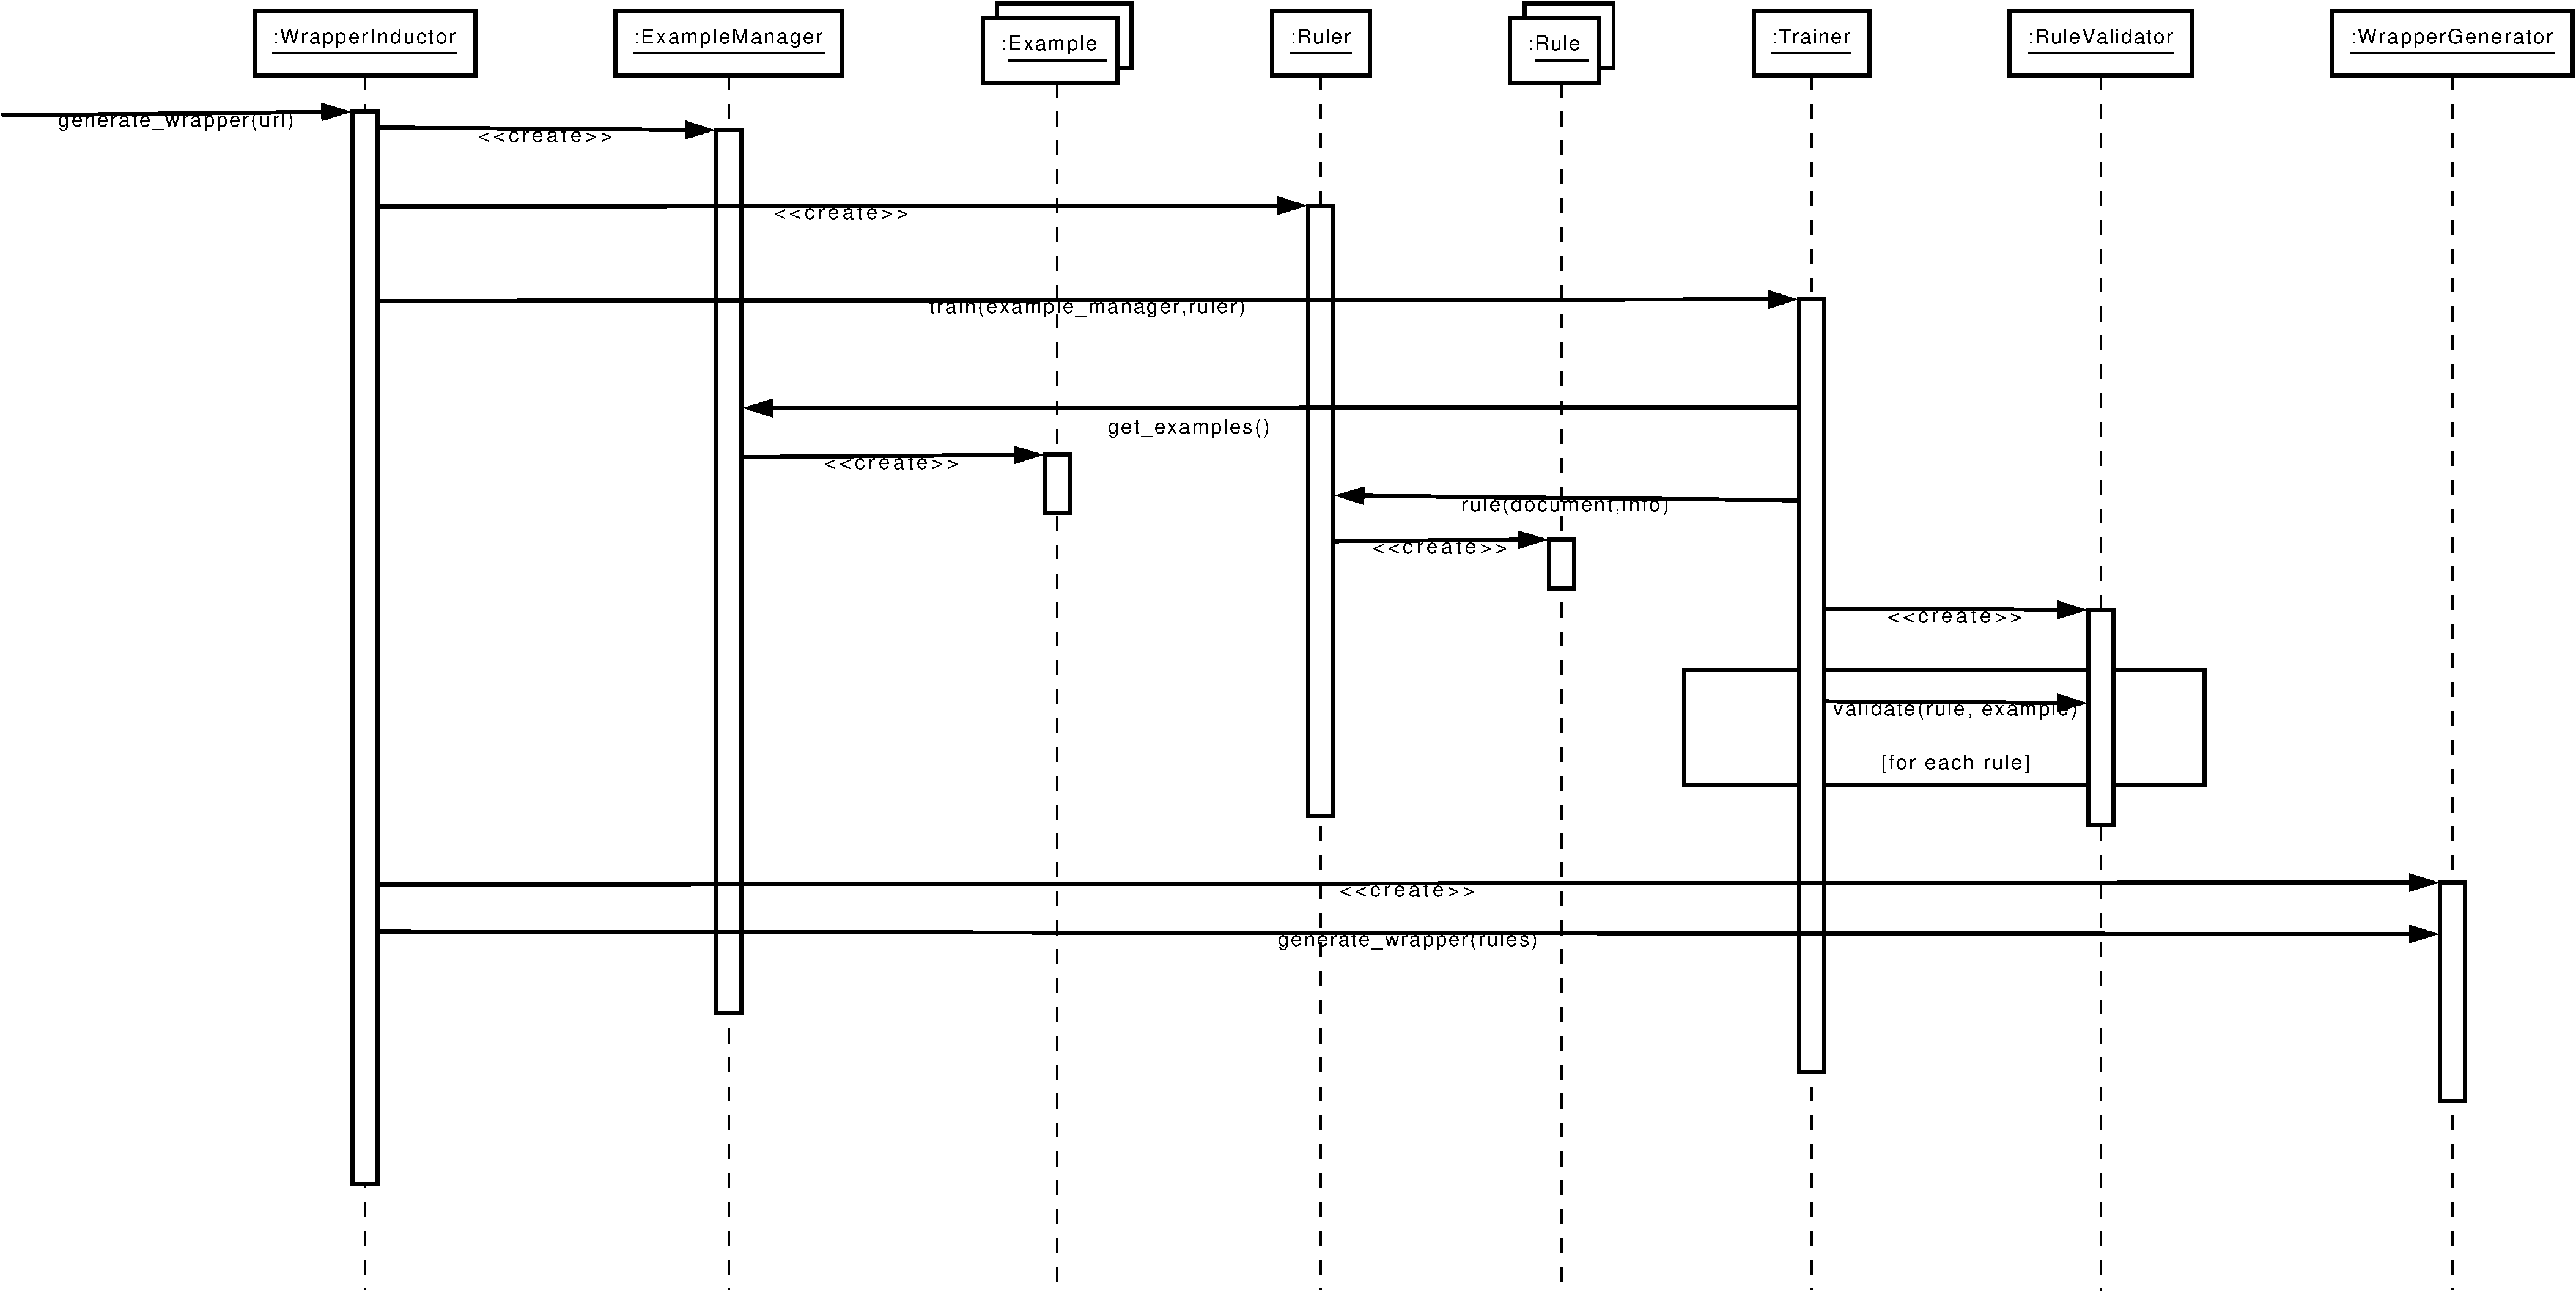
\includegraphics[scale=0.3]{figures/wrapper_induction.pdf}
\caption{Diagrama de seq��ncia}
\end{center}
\end{figure}
\end{landscape}
\end{document}


